\documentclass{llncs}
\usepackage{llncsdoc}
\usepackage{epsfig}

%
\begin{document}
\def\addtocontents#1#2{}%
\def\addcontentsline#1#2#3{}%
\def\markboth#1#2{}%
%
%\title{PGR : A Programming package for Physics Processing Units Generation using an FPGA-Based System}
%\title {Towards Reconfigurable High Performance Computing for scientific many-body simulations}
%\title {PGR : A Software Package for Reconfigurable High Performance Computing}
\title {A Methodology for implementing Reconfigurable Physics Processing Units}

\author{Tsuyoshi Hamada\inst{1}, Naohito Nakasato\inst{1}}

\institute{Computational Astrophysics Group,\\
The Physical and Chemical Research Institute (RIKEN),\\
Wako, Saitama 351-0198, Japan}

\maketitle
%
\begin{abstract}
This paper describes a methodology for implementing FPGA-based
accelerator from a high-level specification in a small special-purpose
language.  The idea is to generate, from a high-level description, (a)
a suitable configuration file for the FPGAs, (b) the C source code for
interfacing with the FPGA-based processors that has been generated,
and (c) a software emulator. The FPGA configuration is build by
combining components from a library of parametrized arithmetic
modules; these modules implement fixed point, floating point and
logarithmic numbers with flexible bitwidth and pipeline stages. To
prove our methodology to be correct, we developed PROGRAPE-3 system as
a target hardware platform and implemented $N$-body calculation
algorithm using PGR.  With the PROGRAPE-3 system of a minimum
composition, we have achieved peak performance of 162 Gflops and
mesured performance of 100 Gflops on actual numerical simulation.
In the FPGA-based high performance computing area,
our methodology and implementation is wonderful for all to others existed.
\end{abstract}
%
\section{Introduction}
%

Recently, scientific computation using FPGAs begins to be a promising
piece of work on an interesting topic. Many reports have been
proposed about scientific computation with FPGAs. Roughly these past
reports can be classified into four topics; (A) hardware
implementations, (B) floating point libraries, (C) aoutomatic module
generation, (D) programming techniquie for generating processor core.

In the topic of (A), PROGRAPE-1(PROgrammable GRAPE-1)\cite{HFKM00} is
an earlier example of the use of a reconfigurable hardware for
scientific computation.  PROGRAPE-1 is an FPBA-based Accelerator(FBA)
for astrophysical many-body simulations. It is implemented with two
Altera EPF10K100 FPGAs. Comparing with modern FPGAs, the EPF10K100 is
old-fashioned and has small density(100k gates per a FPGA). However the
peak performance of calculating gravitational force results in 0.96
Gflops. 

The key point of this work is using the fixed point and short-length
logarithmic number format instead of IEEE standard floating point
format. A processor core of PROGRAPE-1 uses 20-bit fixed point format
in the first stage, 14-bit logarithmic number format(7-bit exponent,
5-bit mantissa, sign flag and non-zero flag) in the inner stages,
56-bit fixed point format in the last stage.  The work of PROGRAPE-1
shows advantage on FPGA-based systems for general purpose systems
which force everyone to use IEEE standard floating point format.

Searching parameter region is very effective for FBAs such as
precision and number format. But the searching is a heavy
task. PROGRAPE-1 and the other related work\cite{LKM02}\cite{SS03}\cite{AKEDC04}
used HDL as system programming language and mentioned the need of
automation the task of programming.

The topic of (B) is to construct the library of parametrized floating
point and other format arithmetic modules.  \cite{JL01}\cite{LCCN03}
presented prametrized floating point adders and
multipliers. \cite{LKM02}\cite{WN04} presented parametrized floating
point square roots and divisions. 

Even if these basic arithmetic units are prepared, It is
insufficient to execute scientific computations.  In most of these
works, square root and divisions are implemented using subtractors and
shifters. This way is not suitable especially in pipelined datapath,
bacause the carry propagation of ripple-carried subtractor becomes long and
a lot of pipeline stages are required for square root and division units.
Increasing carry propagation is a fatal problem even for advanced FPGAs.

Function evaluation units(FEUs) are absolutely needed for this
problem.  FEUs are used for calculating arbitrary functions such as
$\sqrt{x}$, $log(x)$, $x^{-1.5}$ etcelra by table look-up method,
polynomial approximation method, or the hybrid
method\cite{FO01}\cite{M97}.  In general, FEUs for FBAs must be
customizable to treat different functions, function evaluation
methods, or precision according to run-time conditions.  This
customability makes it difficult to implement FEUs into statical HDL
library which realizes customability by HDL's
generic parameters such as \verb|GENERIC| or \verb|ATTRIBUTE|.

The topic of (C) is to generate floating point units dynamically from
some smart software.  Leaving the generation of floating units to a
software, it becomes easy to implement ``troublesome'' arithmetic
units such as FEUs at run-time.  At run-time, a module generation
software recieves parameters such as different functions, function
evaluation methods, precision or pipeline stages which come from user
input or some other high-level software.

There are many types of function evaluation methods for FPGAs or
custom LSIs.  When you consider FPGA implementation, it is an
important factor which methods should be selected.  As the latest
report, Ho\cite{HTYLL03} developed function evaluation generator and
they tried to implement gravitational N-body pipeline.  They works
uses Symmetric Table Addition Method(STAM)\cite{SS99} for table
look-up approximations. In the STAM, the multiplications for polynomial
are replaced by adders and tables. This idea is very exciting and
suitable for old-fashioned FPGAs which have no embeded multiplier and
the STAM can recieve the advantage only to the 1st order
approximation.  Then their implementation will be difficult to apply
to real N-body simulations.  Though it is not the essential matter of
our work, the comparison with our implementations is described in
after section.

Choice of methods for module generation needs careful considerations.
For current advanced FPGAs, DSP blocks are useful for realizing small
multiplications.  And we think the use of embedded RAMs such as Block
RAMs should be used for a cash-memory such as a particle memory unit
in N-body implementation and should not be consumed for coefficient
tables on FEUs.  In the side of precision and logic consumption, the
chebyshev polynomial is more better than polynomials using tayler
series. Using chebyshev polynomial, accuracy becomes more better than
tayler's in FEUs sush as $\log(1+2^{-x})$ and the neccessary order of
polynomial becomes smaller.  Then the size of coeffients table is
relativelly small. Actually we can implement coefficient tables into
small number of logic cells which are called distributed RAMs in
Xilinx devices.

If the floating point units are prepared as libraries or generated
from some software, one needs a deep understanding of details of such
libraries.  Thus, even though the reusability significantly reduce the
amount of the work needed for the second and later design for a
person, the initial hurdle remains rather high, for a person who has
never used such libraries, or actually the availability of the
libraries make the hurdle even higher, since a starter needs to
understand, in addition to the basics of the hardware design and HDL,
the use of such libraries.  Furthermore, a price of libraries is quite
expensive in general for a academic researcher and it is not always
true that there are suitable libraries for one's purpose as explained
above.

The topic of (D) is aimed at solving the above issues of library or
module generator.  In this topics, the main concern is conversion from
high-level language such as C, Java or C++ to FPGA configuration.

PAM-Blox\cite{MMF97} and JHDL\cite{BH98} is one of the first example
to allow module generation from C++ and Java respectively.  PAM-Blox
concentrates on automation and simplicity to explore the design space.
JHDL treats circuits as objects and has an extraordinary, big language
specification.  JHDL has only a few elemental floating point units so
it seems not to be interested in physics computations so much.  

Their common features are emphasizing the importance of automatic
generation of APIs to communicate between FBAs to the host processor
On the most FBA systems, an interface between the FBA and the host
processor should maximize the data transfer rate and minimize latency.
Even if such smart tool generates an FPGA configuration as a prosessor
implementation, an amateur can't necessarily write such high performance
communication software.

Another important problem on the domain specification is architecture
selection. As well as communication software, the performance of a
particular computation is very sensitive to the difference of hardware
architectures. To solve the selection of appropriate architecture, the
work of PAM-Blox proposes a domain specific compiler\cite{MPMF01}.  In
the domain specific compiler, the promising application is limited by
compiler. This way is to the point on the idea that there is no
almighty architecture for any problem and we sympathize with their
ideas very much. 

The way to specify the application domain produces good results for
the tool developer and the tool users.  For the tool developer, the
language specification becomes compact so it can be easy to implement
a compiler that specializes to an application domain if once the
module generator has been completed as a core conponent of a
programming tool.  For the tool users, it becomes clear whether the
tool agrees with a purpose and easy to understand such a comact
language specification.

Because PAM-Blox seems very wonderful tool, we feel they might appeal
more positively and very regrettable not to try to accelerate physics
computations such as gravitational $N$-body simulations or
particle-based hydrodynamics simulations. If they showed it to us, we
might have used their tools.


The work of CAST(Computer Arithmetic Synthesis Tool), however it may
be classified into topic (C), refers implementation of $N$-body
pipeline. The main concern about CAST is just connect modules, and
they doesn't take account for API generation.  In a numerical
calculation, the type conversion and scaling operation are more
confusing than an integer calculation, so implementation of APIs
becomes troublesome inevitably. And as we thought, they make some
serious mistakes in their result\cite{THYL04}.  In \cite{THYL04}, the
figure 12 in page 10 shows the result between GRAPE-3 and their
implementation is inconsistent.  In their figure 12a, the 8-bit
precision of their floaing point implementation is not better accurate
than the GRAPE-3 which uses 5-bit presition. The figure 12c is also
inconsistent. These inconsistencies are due to by mistakes of scaling.
Let us add a few more words for their honor, their modules may be good
in accuracy except whether the modules to be effective.  The
implementation of APIs are wrong.  The developer of the tool has
trouble in executing a collect calculation, no astronomer can use it.



%Implementation of FEUs on FPGAs are 
%reported in \cite{HTYLL03}\cite{}\cite{}. 

%The target of these libraries is mainly HDL environment which is not 
%familiar with general purpose systems who uses fortran or C.


In this paper, we describe details of the PGR package
that makes a design flow of an FBA much simpler than
the conventional design flow.
In section 2, we present a basic idea behind the PGR package
and describe details of our newly developed parametrized 
floating-point arithmetic modules that are key components of the PGR package.
Moreover, we show a simple design example using the PGDL.
In section 3, we describe an example of a real application 
and show obtained performance on the PROGRAPE-3.
Finally, we summarize our results in section 4.
%
\section{PGR : Processors Generator for Reconfigurable systems}
\subsection{Basic idea behind the PGR system}

The main problem with FBAs is that the user need to
develop the detailed hardware design for the processor to be
implemented to FPGA chips. In addition, she or he has to write the
control logic for the processor, communication and data conversion
library on the host processor, and application program which uses the
developed processor. These require detailed knowledge of hardware
design, a hardware description language such as VHDL, the operating
system and the application, and amount of human work is huge. A
relatively simple design would require 1 person-year or more.


\begin{figure*}[htb]
\begin{center}
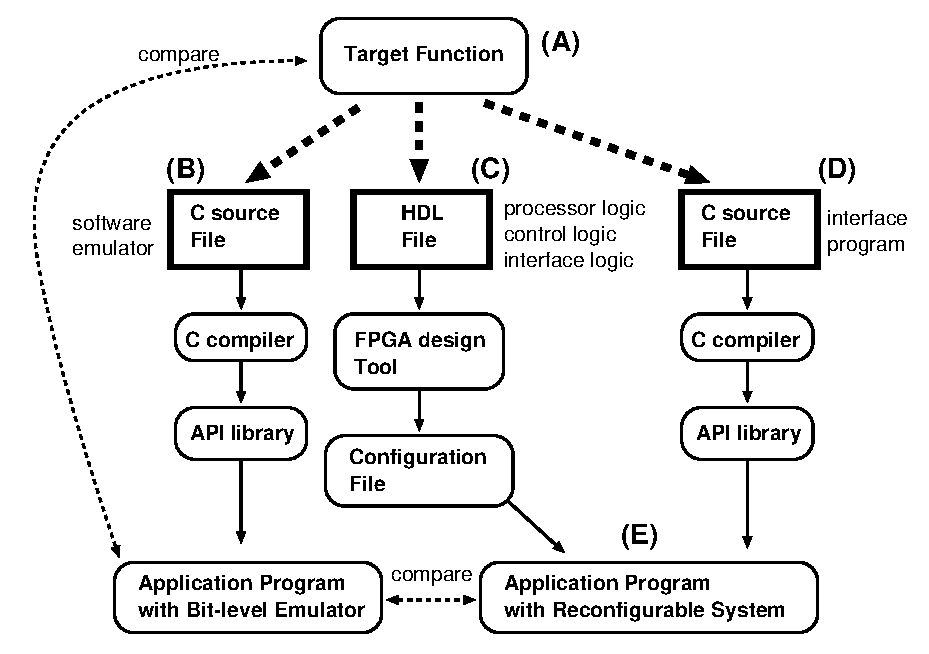
\includegraphics[angle=+0,width=12cm]{./mat/tradflow.eps}
\caption{Conventional work flow for implementing an application on a FBA system.}
\label{tradflow}
\end{center}
\end{figure*}

Figure\ref{tradflow} shows conventional work flow for implementing an application on an FBA.
The work flow consists of the following five steps.

\begin{itemize}
\setlength{\itemsep}{6pt}

\item[(A)] Target Function Specification:
We specify a target function, namely the function that pipeline
processors calculate. This step includes to specify 
data flow for the calculation of the target function, 
and input and output number format and word length for each arithmetic operation. 

\item[(B)] Bit-Level Software Emulator:
We develop a software emulator which implements the target function
defined in step (A). Using this software emulator, we verify
whether the designed hardware can actually calculate the target
function with required accuracy. In this step, we also define the
application program interface (API). 

\item[(C)]  Hardware Design:
In this step, we actually write the source code which implements the
pipeline processors in a hardware description language (HDL) such as VHDL.
In addition, we design the control logic and host interface logic also
in some HDL. The HDL description is compiled to the configuration data
for the FPGAs by a CAD software, usually provided by the
manufacturer of the FPGA device.

\item[(D)] Interface Software:
We develop the software on the host computer which takes care of the
communication to the FBA and data format conversion between the
floating-point data on the host and specialized data format used on
the developed pipeline processors. The developed software should have
the same API as that of the software emulator developed in step (B).

\item[(E)] Finally, we can actually use the FBA with
real application program.
\end{itemize}

In these steps, we have to design, test, and debug a large amount of
hardware logics and softwares. Of course, many of the softwares and
hardware designs can be reused, when we develop different
applications. For example, the design of the floating-point multiplier
is rather generic, and can be used in almost any application. Also, it
is possible to buy IP cores of such designs.

However, just to understand how to use the IP cores, one need a deep understanding
of details of the IP cores. Thus, even
though the reusability significantly reduce the amount of the work
needed for the second and later design for a person, the initial
hurdle remains rather high, for a person who has never used 
such IP core, or actually the availability of the IP cores make the hurdle
even higher, since a starter needs to understand, in addition to the
basics of the hardware design and HDL, the use of such IP cores.
Furthermore, a price of IP cores is quite expensive in general for a academic 
researcher and it is not always true that there are suitable IP cores
for one's purpose as explained above.

The development of a communication software is generally even more
difficult than the design of the hardware, since it requires the
knowledge of how a device driver work in the operating
system of the host computer, and infinite number of small details;
how to integrate the device driver to the operating system, how to
correctly generate the compiler flags to compile the device driver and so on.
All these works combined make it almost impossible 
for possible users to even think of implementing the pipeline processor on an FBA.

In theory, most of the softwares and hardware descriptions,
including the bit-level design of the pipeline processors itself,
can be automatically generated from some high-level description of the
pipeline. The basic idea behind the PGR package,
which we will describe details in this paper,
is to provide such automatic generation.
The PGR package analyzes a description of pipeline processors
written in the PGR Description Language (PGDL) as input
and then translates and generates necessary hardware descriptions, 
a bit-level emulator, and communication softwares.
Namely, a possible user of an FBA can concentrate on writing their
application in the PGDL.
This means that the PGR system can drastically reduce the amount of
the work (and needed knowledge) of such user.
More importantly, the PGDL does not depends on a specific hardware
(e.g., PROGRAPE-3) and this make it possible to
reuse a application written in the PGDL on a newly developed FBA
when the PGR package supports the new FBA.
The effort spent to design one application on
one hardware will not be thrown away when a new hardware becomes available.

The PGR software generates all necessary design descriptions, except for
the application software itself, from a high-level design description
of the pipeline processor in the PGR language. The PGR language is a
simple language, specialized to the description of pipeline
processors. Thus, the design of pipeline processor in PGR language is
much easier than the traditional design. For real applications such as
the pipeline for gravitational interaction, the pipeline processor
generated by PGR achieved the performance similar to that of
hand-written code. 
This paper describes a methodology of PGR and the implementation result on real hardware.

If we inspect Figure \ref{tradflow} again, we can see the fact that
{\bfseries all} softwares and hardware description is derived from the
target function specification in step (A). Thus, it should be possible
for a sufficiently smart software to generate all necessary softwares
and hardware descriptions from the target function description written
in some high-level language. The basic idea of PGR is to develop such
a smart software.

\begin{figure*}[htb]
\begin{center}
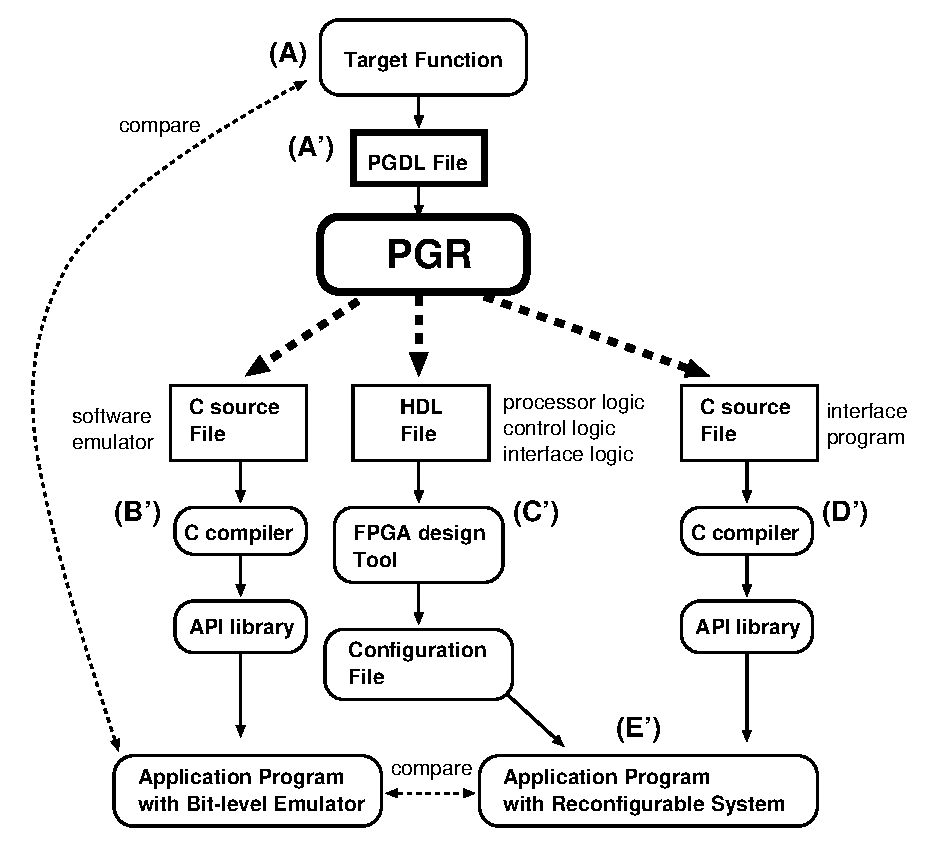
\includegraphics[angle=+0,width=12cm]{./mat/pgrflow.eps}
\caption{How the design flow changes with PGR.}
\label{pgrflow}
\end{center}
\end{figure*}

Figure \ref{pgrflow} shows how the design flow changes with the PGR package.
After we define a target function, then we write it in the PGDL
(see the later section for details on the PGDL).
The PGR software system takes this PGDL description of the pipeline processors
as input, and generates all softwares and hardware descriptions.
Thus, with the PGR package, a user do not have to write HDL source codes for
the processor and C source codes for a communication software.

\subsection{PGR five layers model}
To make the PGR software system independent on a specific hardware,
we create the PGR five layers model which divide 
an FBA into five parts.
Figure \ref{fig5model} shows the PGR five layers model, 
and it's composed of User Program Layer(UPL), API Layer(APL),
Device Driver Layer(DDL), I/O \& Control Logic Layer(ICL) and
Arithmetic Logic Layer(ALL).

The UPL is a user application which communicates
with an FBA through the APL.
The APL contains the top level API implementations that
doesn't depend on an individual FBA.
The DDL consists of both a low level communication library and a device driver software. 
The ICL is a glue logic such as the PCI interface logic and 
local I/O logic on an FBA.
The ALL is composed of parametrized arithmetic modules,
details of which is described later, 
and control logic of pipeline processors.

The PGR package generates only the layers that doesn't depend on 
a specific FBA, namely the APL and ALL.
The others layers (DDL and ICL) depend on hardware specification
of the FBA such as architecture of a host computer, used operating
system, or a type of inter-connection hardware (e.g., PCI, PCI-Express and so on).
We define standard specifications between the hardware depended layers(DDL,ICL)
and the independent layers(APL,ALL).
Our current target hardware is the PROGRAPE-3 board (see figure\ref{figpg3}).
The inter-connection hardware of the PROGRAPE-3 is the 66 MHz, 64 bit PCI bus
and detailed implementation of the ICL for PROGRAPE-3
is shown in Figure\ref{figicl}.

\begin{figure}[htb]
\begin{center}
  \begin{minipage}{.45\linewidth}
    \begin{center}
    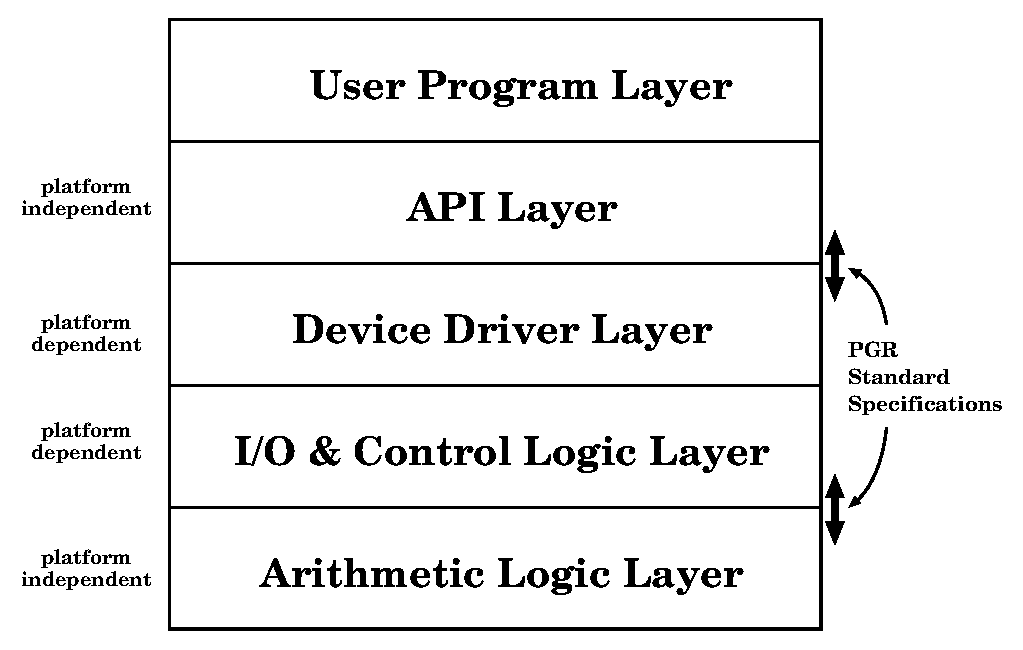
\includegraphics[angle=+0, width=1.2 \linewidth]{./mat/5model.eps}
    \caption{PGR five layers model.}
    \label{fig5model}
    \end{center}
  \end{minipage}
  \hspace{2.4pc}
  \begin{minipage}{.45\linewidth}
    \begin{center}
    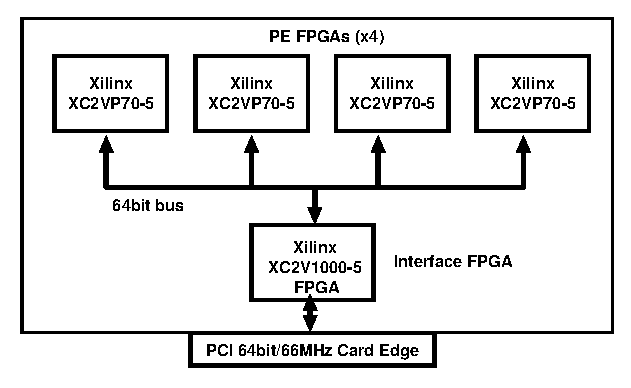
\includegraphics[angle=+0,width=1.2 \linewidth]{./mat/pg3.eps}
    \caption{PROGRAPE-3 board structure}
    \end{center}
  \end{minipage}
\end{center}
\end{figure}



\begin{figure}[htb]
\begin{center}
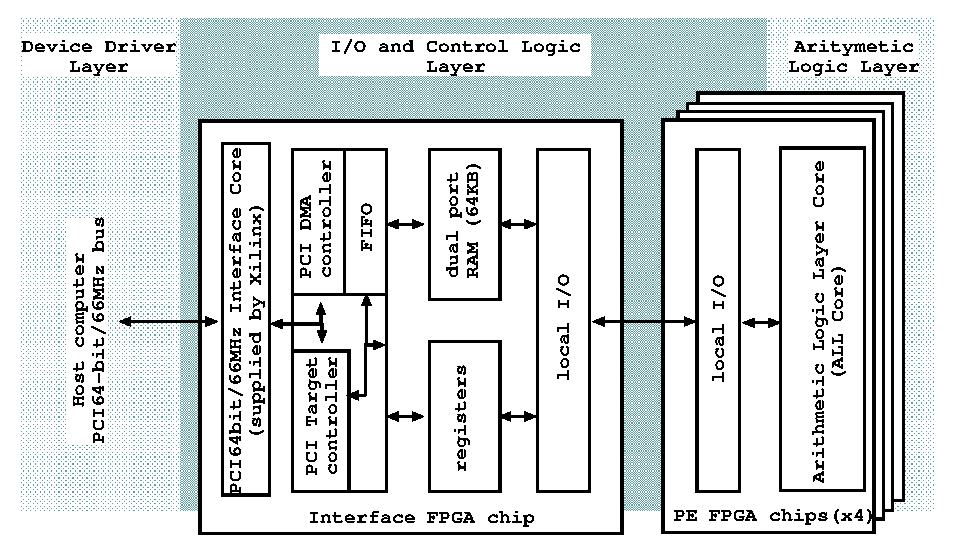
\includegraphics[angle=+0,width=8cm]{./mat/pgr_icl.eps}
\caption{real implementation of ICL.}
\label{figicl}
\end{center}
\end{figure}

\subsection{Parametrized Arithmetic Modules}
The parametrized arithmetic modules are the most low-level components
for the PGR package such as addition, subtraction, 
multiplication, division, and square-root, etc. 
Currently, the PGR package supports
29 parametrized arithmetic modules as shown in table \ref{tabpgmod}.

In this table, modules with {\tt pg\_float} are floating point format arithmetics.
We define internal floating-point format as 1-bit for a sign, 
1-bit for a non-zero expression, $n$-bit for exponent, 
and $m$-bit for mantissa, where $m$ and $n$ can be 
changed arbitrary up to single-precision for floating-point in the PGDL.
For example, in the PGDL, we can use float-point addition
as follows;
\begin{verbatim}
pg_float_add(x,y,z,26,16,1);
\end{verbatim}
Here, the arguments inside of parentheses indicate
the first input, the second input, output, total bit-length
of floating-point format, bit-length for mantissa,
and number of pipeline stages, respectively,
from the first to sixth argument.
This particular example expresses 
$z = x + y$, where $x,y,z$ are 26-bit floating numbers (mantissa is 16-bit).
And a number of pipeline stage for this arithmetic is one.
We note that for the rounding operation in the PGR package,
we have implemented nine types of several options that
also can be changed by a hidden argument in the PGDL.
If this argument is omitted like above example, 
a rounding to the nearest even is selected.

\begin{table}
\caption{PGDL Parametrized Arithmetic Modules}
\begin{center}
\begin{tabular}{ll}
\hline
\hline
Parametrized Arithmetic Module &  arithmetic\\
\hline
floating point format & \\
 {\tt pg\_float\_add}           &  $+$\\
 {\tt pg\_float\_unsigned\_add} &  $+$ (unsigned)\\
 {\tt pg\_float\_sub}           &  $-$\\
 {\tt pg\_float\_unsigned\_sub} &  $-$ (unsigned)\\
 {\tt pg\_float\_mult}          &  $\times$\\
 {\tt pg\_float\_div}           &  $/$ \\
 {\tt pg\_float\_sqrt}          &  $\sqrt{x}$ \\
 {\tt pg\_float\_square}        &  $x^2$\\
 {\tt pg\_float\_recipro}       &  $x^{-1}$\\
 {\tt pg\_float\_negate}        &  $\times -1.0$\\
 {\tt pg\_float\_compare}       &  compare\\
 {\tt pg\_float\_compare\_abs}  &  compare\\
 {\tt pg\_float\_compz}         &  compare to 0\\
 {\tt pg\_float\_compz\_abs}    &  compare to 0\\
 {\tt pg\_float\_accum}         &  accumulate\\
 {\tt pg\_float\_unsigned\_accum}&  accumulate (unsigned)\\
 {\tt pg\_float\_fixaccum}      &  accumulate\\
fixed point format & \\
 {\tt pg\_fix\_addsub}          &  $+$, $-$\\
 {\tt pg\_fix\_mult}            &  $\times$\\
 {\tt pg\_fix\_unsigned\_mult}  &  $\times$ (unsigned)\\
 {\tt pg\_fix\_accum}           &  accumulate\\
logarithmic format& \\
 {\tt pg\_log\_add}             &  $+$\\
 {\tt pg\_log\_unsigned\_add}   &  $+$ (unsigned)\\
 {\tt pg\_log\_muldiv}          &  $\times$, $/$\\
 {\tt pg\_log\_shift}           &  $\sqrt{x}$, $x^2$\\
format conversion & \\
 {\tt pg\_conv\_fixtofloat}     &  fix $\Rightarrow$ float\\
 {\tt pg\_conv\_floattofix}     &  float $\Rightarrow$ fix\\
 {\tt pg\_conv\_ftol}           &  fix $\Rightarrow$ log\\
 {\tt pg\_conv\_ltof}           &  log $\Rightarrow$ fix\\
\hline
\hline
\end{tabular}
\end{center}
\label{tabpgmod}
\end{table}

Modules {\tt pg\_fix\_addsub} and {\tt
pg\_fix\_accum} are fixed point format adder/subtracter and
accumulator, respectively.  Modules {\tt pg\_log\_muldiv} and {\tt
pg\_log\_unsigned\_add} are logarithmic format multiplier/divider and
unsigned adder, respectively. In the logarithmic format, a positive,
non-zero real number $x$ is represented by its base-2 logarithm $y$ as
$x=2^{y}$.
This logarithmic format is useful because 
it has larger dynamics length for the same word length and
operation such as multiplication and square root
are easier to implement than in the usual floating-point format.
As a result, the logarithmic format has been adapted for the
gravitational pipelines in low-accuracy type GRAPE-1,3,5 systems.
For more details of the logarithmic format, see GRAPE-5 paper
\cite{KFMT00}.
Module {\tt pg\_log\_shift} is a logarithmic format
shifter. Shift operations in the logarithmic format express square
(left shift) and squared root (right shift). 

Modules with {\tt pg\_conv} are converters from a particular format
into another format, e.g., {\tt pg\_conv\_floattofix} converts
a floating-point number into a corresponding fixed point number.

In tables \ref{tabpg_float_mult}, \ref{tabpg_float_unsigned_add},
\ref{tabpg_float_sqrt}, \ref{tabpg_float_recipro},
\ref{tabpg_log_unsigned_add}, and \ref{tabpg_fix_accum}, we illustrate
resource consumption and clock frequency of several important
parametrized arithmetic modules.
Despite we have implemented all of the parametrized arithmetic modules
from full scratch by ourself, 
the obtained performance results for each module
are almost same as other good implementations such as Manheim's (\cite{LKM02}).



\begin{table}
  \begin{center}
    \begin{minipage}{.45\linewidth}
      \caption{Multiplier(floating point)}
      \begin{center}
	\begin{tabular}{cccrr}
	  \hline
	  \hline
	  length  & length(mantissa) & stages & MHz & slices\\
	  \hline
	  18   &  9 & 2 & 290.192 &  31 \\
	  &    & 0 & 133.387 &  15 \\
	  \hline
	  26   & 17 & 4 & 224.266 &  56 \\
	  &    & 2 & 151.953 &  41 \\
	  &    & 0 &  80.762 &  23 \\
	  \hline
	  33   & 24 & 3 & 136.986 &  93 \\
	  &    & 0 &  68.847 &  56\\
	  \hline
	  \hline
	\end{tabular}
      \end{center}
      \label{tabpg_float_mult}
    \end{minipage}
    \hspace{2.4pc}
    \begin{minipage}{.45\linewidth}
      \caption{Multiplier(floating point)}
      \begin{center}
	\begin{tabular}{cccrr}
	  \hline
	  \hline
	  length  & length(mantissa) & stages & MHz & slices\\
	  \hline
	  18   &  9 & 2 & 290.192 &  31 \\
	  &    & 0 & 133.387 &  15 \\
	  \hline
	  26   & 17 & 4 & 224.266 &  56 \\
	  &    & 2 & 151.953 &  41 \\
	  &    & 0 &  80.762 &  23 \\
	  \hline
	  33   & 24 & 3 & 136.986 &  93 \\
	  &    & 0 &  68.847 &  56\\
	  \hline
	  \hline
	\end{tabular}
      \end{center}
      \label{tabpg_float_mult}
    \end{minipage}
  \end{center}

  \begin{center}
    \begin{minipage}{.45\linewidth}
      \caption{Square root (floating point)}
      \begin{center}
	\begin{tabular}{cccrr}
	  \hline
	  \hline
	  length  & length(mantissa) & stages & MHz & slices\\
	  \hline
	  18   &  9 & 4 & 215.517 & 86 \\
	  &    & 2 & 157.754 & 71 \\
	  &    & 0 &  79.971 & 51 \\
	  \hline
	  26   & 17 & 4 & 188.964 & 140 \\
	  &    & 2 & 127.959 & 116 \\
	  &    & 0 &  56.500 &  84 \\
	  \hline
	  33   & 24 & 5 & 141.243 & 425 \\
	  &    & 3 & 104.998 & 392 \\
	  &    & 1 &  70.210 & 374 \\
	  \hline
	  \hline
	\end{tabular}
      \end{center}
      \label{tabpg_float_sqrt}
    \end{minipage}
    \hspace{2.4pc}
    \begin{minipage}{.45\linewidth}
      \caption{Adder (logarithmic number)}
      \begin{center}
	\begin{tabular}{cccrr}
	  \hline
	  \hline
	  length  & length(mantissa) & stages & MHz & slices\\
	  \hline
	  14   &  6 & 4 & 201.077 & 94 \\
	  &    & 2 & 151.207 & 73 \\
	  &    & 0 &  64.545 & 57 \\
	  \hline
	  17   &  9 & 5 & 195.369 & 116 \\
	  &    & 2 & 138.042 &  92 \\
	  &    & 0 &  58.828 &  86 \\
	  \hline
	  20   & 12 & 6 & 218.293 & 191 \\
	  &    & 2 & 135.125 & 123 \\
	  &    & 0 &  53.562 & 115 \\
	  \hline
	  \hline
	\end{tabular}
      \end{center}
      \label{tabpg_log_unsigned_add}
    \end{minipage}
  \end{center}
\end{table}


\subsection{PGDL: PGR Description Language}
In this subsection, we illustrate how pipeline processors are
specified in the PGDL and how such description is translated
into the hardware description of pipelined processors.

\begin{figure}[htb]
\begin{center}
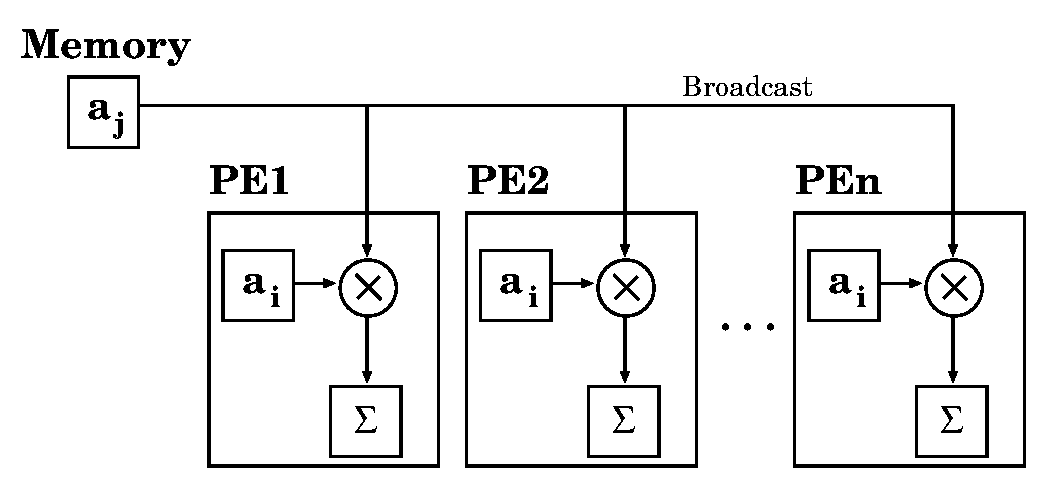
\includegraphics[angle=+0,width=8cm]{./mat/simple.eps}
\caption{Block diagram of the example processors(PEs).}
\label{fig4}
\end{center}
\end{figure}

With the current version of the PGR package, it is specially tuned
to generate hardware description of pipelined processors
for the following summation form;
\begin{equation}
f_i = \sum_{j = 1}^{n} F(\boldmath{p}_i, \boldmath{p}_j),
\end{equation}
where $f_i$ is summation for $i$-th data, $\boldmath{p}_i$ are
some values associated with $i$-th data, and
$F$ expresses calculations where $i$-th and $j$-th data are as inputs.

As an example target, we consider the following artificial calculations;
\begin{equation}
f_i = \sum_j^n {a_i a_j}.\qquad (i=1,...,n)
\end{equation}
Figure \ref{fig4} shows the block diagram
for this target processor.
Here, $a_i$ and $a_j$ are scalar values for $i$-th and
$j$-th elements, respectively.
This target simply calculates a product of $a_i$ and $a_j$, 
and sums the product up for all $j$.
In this example, we have the essential ingredients of an FBA:
data, their representation, functional form of arithmetic operations
between data $i$ and $j$.

Figure \ref{fig5} shows the PGDL description of this target function.
The first two lines define the bit-length of the floating-point format.
These definitions are actually used in the next block
(three lines starting with ``/''),
which defines the register and memory layout,
which also determine the interface API etc. 
For the data $a_i$ (and $a_j$), we use a floating point format,
with 26 bits in total (1-bit for sign, 1-bit for non-zero flag, 8-bits
for exponent, and 16-bits for mantissa).
The line ``/NPIPE'' specifies a number pipeline processors (10 processors in this case).
The final part describes the target function itself using
parametrized arithmetic modules. It has C-like appearance, but
actually defines the hardware modules and their interconnection.

From such PGDL description, the following ALL (as shown in figure \ref{fig4})
is generated; the $i$-th data is stored in the on-chip memory,
and new data ($j$-th data) is supplied at each clock cycle.
The $i$-th data is unchanged during one calculation, and 
the result ($f_i$) is stored in the register.

\begin{figure}
\scriptsize
\begin{verbatim}
#define NFLO 26
#define NMAN 16

/JPSET x,  aj[], float, NFLO, NMAN;
/IPSET y,  ai[], float, NFLO, NMAN;
/FOSET z,  fi[], float, NFLO, NMAN;

/NPIPE 10;

pg_float_mult      (x,   y,  xy, NFLO, NMAN, 1);
pg_float_accum     (xy,  z,      NFLO, NMAN, 1);
\end{verbatim}
\caption{An example of design entry file written in PGDL}
\label{fig5}
\end{figure}


\section{Application}
To show the possibility of the PGR package, we have implemented gravitational
force pipeline for astrophysical $N$-body simulations.

The implemented pipeline processors calculate gravitational force 
$\mathbf{a}_i$ of $i$-th particle exerted by all other particles:
\begin{equation}
\mathbf{ a}_i = \sum_j {m_j \mathbf{ r}_{ij} \over (r_{ij}^2 + \varepsilon^2)^{3/2}}
\end{equation}
where $\mathbf{r}_{ij}$ is a distance between $i$ and $j$-th particles
($\mathbf{r}_j - \mathbf{r}_i $), 
$m_{j}$ is mass of $j$-th particle, and $\varepsilon$ is a softening parameter
that prevents a zero-division.

Figure \ref{figgravfloat_pgdl} and \ref{figgrav5_pgdl}
show PGDL descriptions for this gravitational force pipeline
using 26-bit floating point arithmetic operations and
17-bit logarithmic arithmetic operations, respectively.
Note there are a several differences between two descriptions.

Figure \ref{fig_grav_float_nodelay} shows a generated 
data flow graph that corresponds to the floating-point pipeline.
Since all operations must be synchronized in pipeline processors, 
a module in the PGR package automatically inserts
delay registers for synchronization.
Figure \ref{fig_grav_float_delay} shows a data flow
after the delay registers, which are indicated by bold solid circles, are inserted.

We have compared this two implementations with the GRAPE-5 as the
existing implementation.  Table \ref{tabcompg5} shows the result of
the comparison.  In the case of the floating-point implementation
(\ref{figgravfloat_pgdl}), 24 pipeline processors can be successfully
implemented on one PROGRAPE-3 board, while in the case of the
logarithmic implementation (\ref{figgrav5_pgdl}), which is actually
equivalent with the GRAPE-5, 64 pipelines can be successfully
implemented.  In both cases, each pipeline processors successfully
operate at 66.6MHz.  The number of floating-point operations per one
interaction is 38.  Thus the peak speed of one PROGRAPE-3 board is
60.8 Gflops with 26-bit floating-point arithmetics and 162.1 Gflops
with 17-bit logarithmic arithmetics.
In the case of same accuracy, the performance of our implementation on one PROGRAPE-3
board is five times faster than one GRAPE-5 board.  And even if we use
twice the accuracy, the performance of our implementation is the still
two times good than the GRAPE-5.

Figure \ref{MESURE-PERFORM} shows the mesured calculation speed of
single PROGRAPE-3 board with 17-bit logarithmic arithmetics.  The
horizontal axis means the number of particles.  The vertical axis
means the mesured speed for the direct-summation algorithm.  Because
the order of the calculation and communication is $O(N^2)$ and $O(N)$
respectively, the mesured speed approaches the peak speed as the
number of particles increases.

\begin{figure}
\scriptsize
{\tiny
\begin{verbatim}
 1 /* -------------------------------------------------- MACRO */
 2 #define NFLO 26
 3 #define NMAN 16
 4 #define NFIX 57
 5 #define NACC 64
 6 #define FOFFSET (131072.0)
 7 #define NST_MULT 2
 8 /* ----------------------------------------- I/O DEFINITION */
 9 /JPSET xj[3], x[][],  float, NFLO, NMAN;
10 /JPSET mj,    m[],    float, NFLO, NMAN;
11 /IPSET xi[3], x[][],  float, NFLO, NMAN;
12 /IPSET ieps2, eps2,   float, NFLO, NMAN;
13 /FOSET sx[3], a[][],  fix,   NACC, (-1.0/FOFFSET);
14 /CONST_FLOAT fofst, FOFFSET, NFLO, NMAN;
15
16 /NPIPE 6;
17 /* ------------------------------------------- PE DATA FLOW */
18 pg_float_sub(xi,xj,   dx,  NFLO,NMAN,4);
19 pg_float_mult(dx,dx, dx2,           NFLO,NMAN, NST_MULT);
20 pg_float_unsigned_add(dx2[0],dx2[1], x2y2,  NFLO,NMAN,4);
21 pg_float_unsigned_add(dx2[2],ieps2,  z2e2,  NFLO,NMAN,4);
22 pg_float_unsigned_add(x2y2,z2e2,r2, NFLO,NMAN, 4);// x2y2+z2e2
23 pg_float_sqrt(r2,r1,       NFLO,NMAN, 3);        // sqrt(r2)
24 pg_float_recipro(r1,r1i ,  NFLO,NMAN, 2);        // 1/r1
25 pg_float_mult(r1i,r1i,r2i, NFLO,NMAN, NST_MULT); // r1i * r1i
26 pg_float_mult(r1i,r2i,r3i, NFLO,NMAN, NST_MULT); // r1i * r2i
27 pg_float_mult(r3i,mj,mf,   NFLO,NMAN, NST_MULT); // r3i * mj
28 pg_float_mult(mf,fofst,mfo,NFLO,NMAN, NST_MULT); // mf  * fofst
29 pg_float_mult(mfo,dx,fx,   NFLO,NMAN, NST_MULT); // mfo * dx[]
30 pg_conv_floattofix(fx,ffx, NFLO,NMAN,NFIX,1); // fxo[] -> ffx[]
31 pg_fix_accum(ffx,sx,       NFIX, NACC, 4);    // sx[] += ffx[]
\end{verbatim}
}
\caption{a PGDL for gravitational force calculation (using 26-bit floating point arithmetics)}
\label{figgravfloat_pgdl}
\end{figure}

\begin{figure}
\scriptsize
{\tiny
\begin{verbatim}
 1 /* -------------------------------------------------- MACRO */
 2 #define NPOS 32
 3 #define NLOG 17
 4 #define NMAN 8
 5 #define NCUT 6
 6 #define NFOR 57
 7 #define NACC 64
 8 #define xsize (100.0)
 9 #define mmin (1.220703125e-04)
10 #define xoffset (xsize/2.0)
11 #define xscale (pow(2.0,(double)NPOS)/xsize)
12 #define mscale (pow(2.0,95.38)/mmin)
13 #define escale (xscale*xscale)
14 #define foffset (pow(2.0,23.0))
15 #define fscale (-xscale*xscale*foffset/mscale)
16 /* ----------------------------------------- I/O DEFINITION */
17 /NPIPE 17;
18
19 /JPSET xj[3], x[][], ufix,      NPOS,xscale,xoffset;
20 /JPSET mj,    m[],   log,       NLOG,NMAN,mscale;
21 /IPSET xi[3], x[][], ufix,      NPOS,xscale,xoffset;
22 /IPSET ieps2, eps2,  log,       NLOG,NMAN,escale;
23 /FOSET sx[3], a[][], fix,       NACC,fscale;
24 /CONST_LOG fx_ofst,  8388608.0, NLOG, NMAN, 1.0;
25 /* ------------------------------------------- PE DATA FLOW */
26 pg_fix_addsub(SUB,xi,xj,xij,NPOS, 1);
27 pg_conv_ftol(xij,dx,NPOS,NLOG,NMAN, 2);
28 pg_log_shift(1,dx,x2,NLOG);
29 pg_log_unsigned_add_itp(x2[0],x2[1], x2y2,   NLOG,NMAN,4, NCUT);
30 pg_log_unsigned_add_itp(x2[2],ieps2, z2e2,   NLOG,NMAN,4, NCUT);
31 pg_log_unsigned_add_itp(x2y2,z2e2,   r2,     NLOG,NMAN,4, NCUT);
32 pg_log_shift(-1,r2,       r1,        NLOG);
33 pg_log_muldiv(MUL,r2,r1,  r3,        NLOG,1);
34 pg_log_muldiv(DIV,mj,r3,  mf,        NLOG,1);
35 pg_log_muldiv(MUL,mf,dx,  fx,        NLOG,1);
36 pg_log_muldiv(SDIV,fx,fx_ofst, fxo,  NLOG,1);
37 pg_conv_ltof(fxo,  ffx,              NLOG,NMAN,NFOR,2);
38 pg_fix_accum(ffx,  sx,               NFOR,NACC,1);
\end{verbatim}
}
\caption{a PGDL for gravitational force calculation (using 17-bit logarithmic arithmetics)}
\label{figgrav5_pgdl}
\end{figure}

\begin{figure}[htb]
\begin{center}
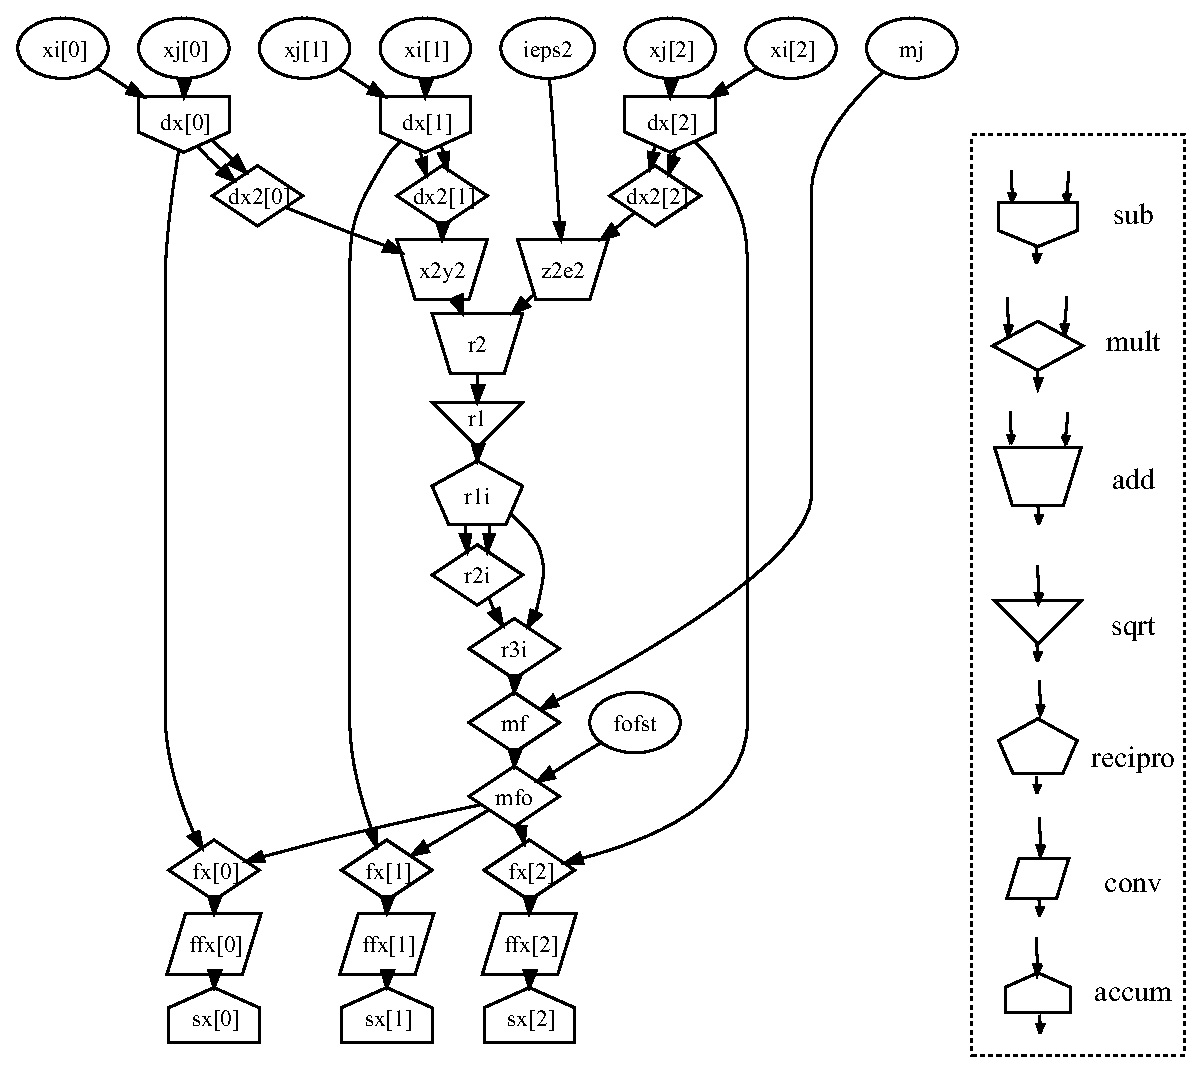
\includegraphics[angle=+0,width=8cm]{./mat/grav_float_nodelay.eps}
\caption{Simple data flow of gravitational force pipeline.}
\label{fig_grav_float_nodelay}
\end{center}
\end{figure}

\begin{figure}[htb]
\begin{center}
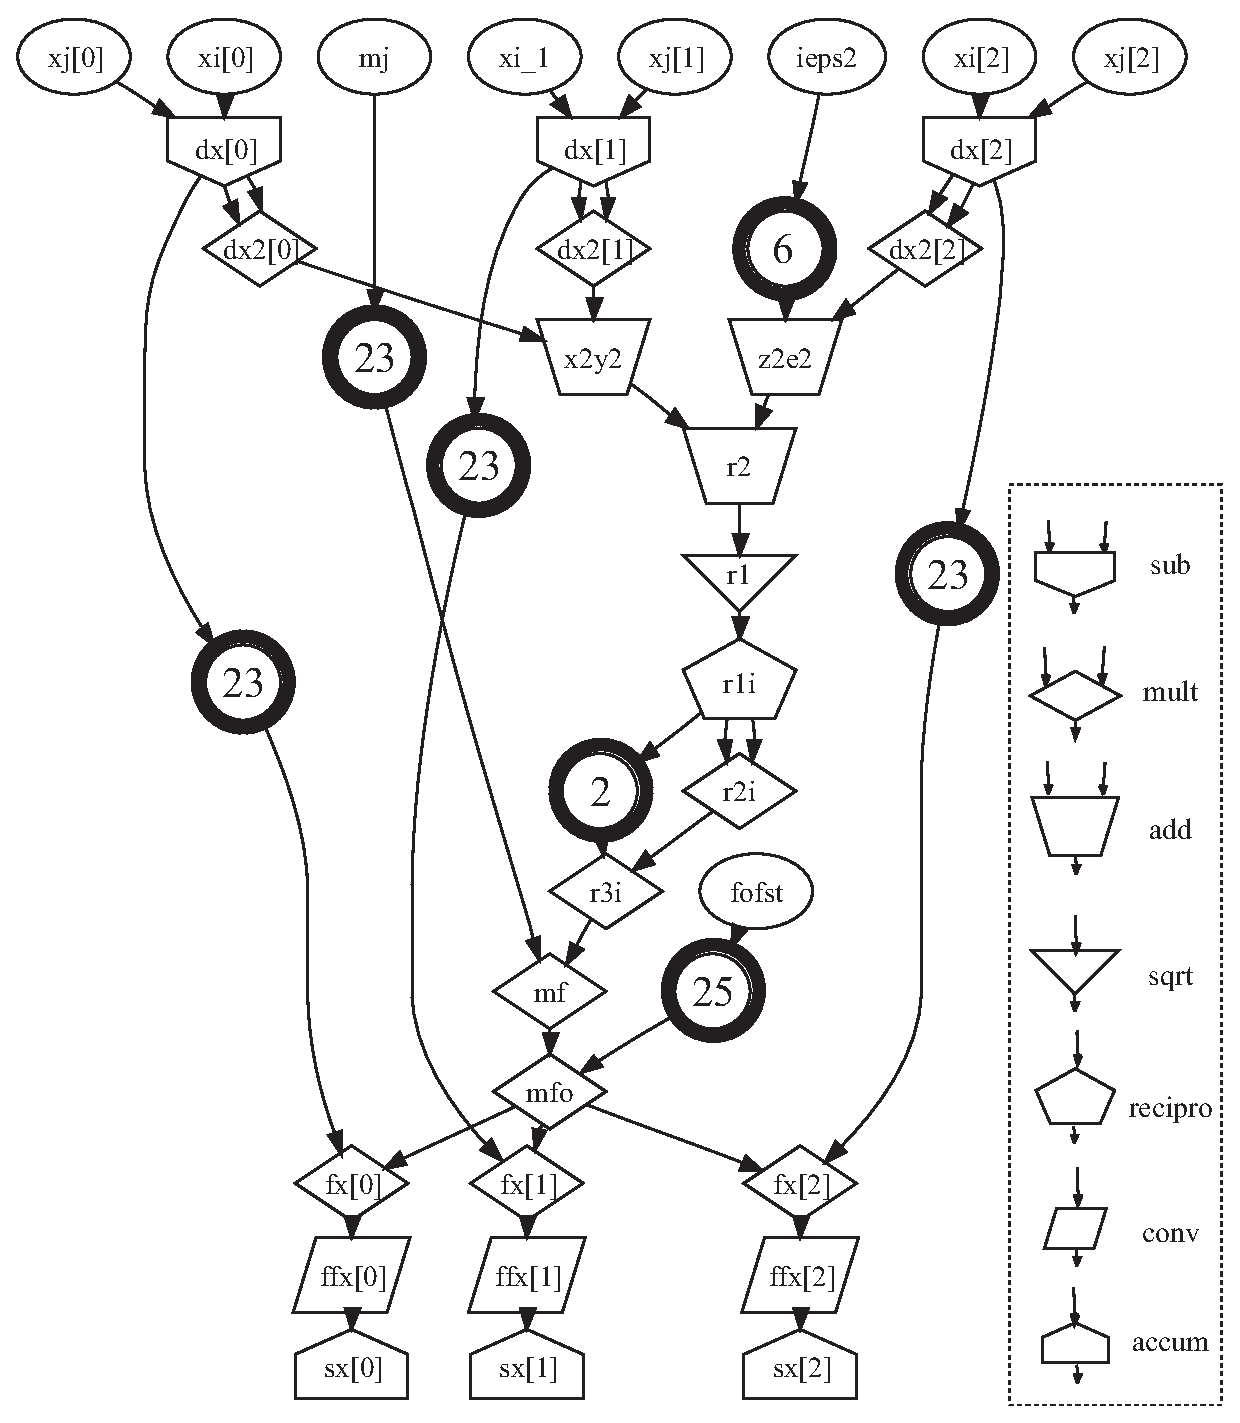
\includegraphics[angle=+0,width=8cm]{./mat/grav_float_delay.eps}
\caption{Delay inserted data flow of gravitational force pipeline.}
\label{fig_grav_float_delay}
\end{center}
\end{figure}


\begin{table*}
\caption{Implementation result and comparison with other implementation}
\begin{center}
\begin{tabular}{lccc}
\hline
\hline
                     & GRAPE-5 board(8 ASICs) & \multicolumn{2}{c}{PROGRAPE-3 board(4 FPGAs)}  \\
\hline
format :input        & 32-bit fixed point  & 26-bit floating point & 32-bit fixed point \\
format :internal     & 17-bit logarithmic  & 26-bit floating point & 17-bit logarithmic \\
format :accumulation & 64-bit fixed point  & 64-bit fixed point    & 64-bit fixed point \\
A number of PEs      & 16                  &   24                  &   64               \\
perk performance(Gflops)    & 48.6         & 60.8                  & 162.1              \\
pair-wise error             & 10$^{-2.4}$   &  10$^{-4.8}$ & 10$^{-2.4}$                \\

\hline
\hline
\end{tabular}
\end{center}
\label{tabcompg5}
\end{table*}

\begin{figure}[htb]
\begin{center}
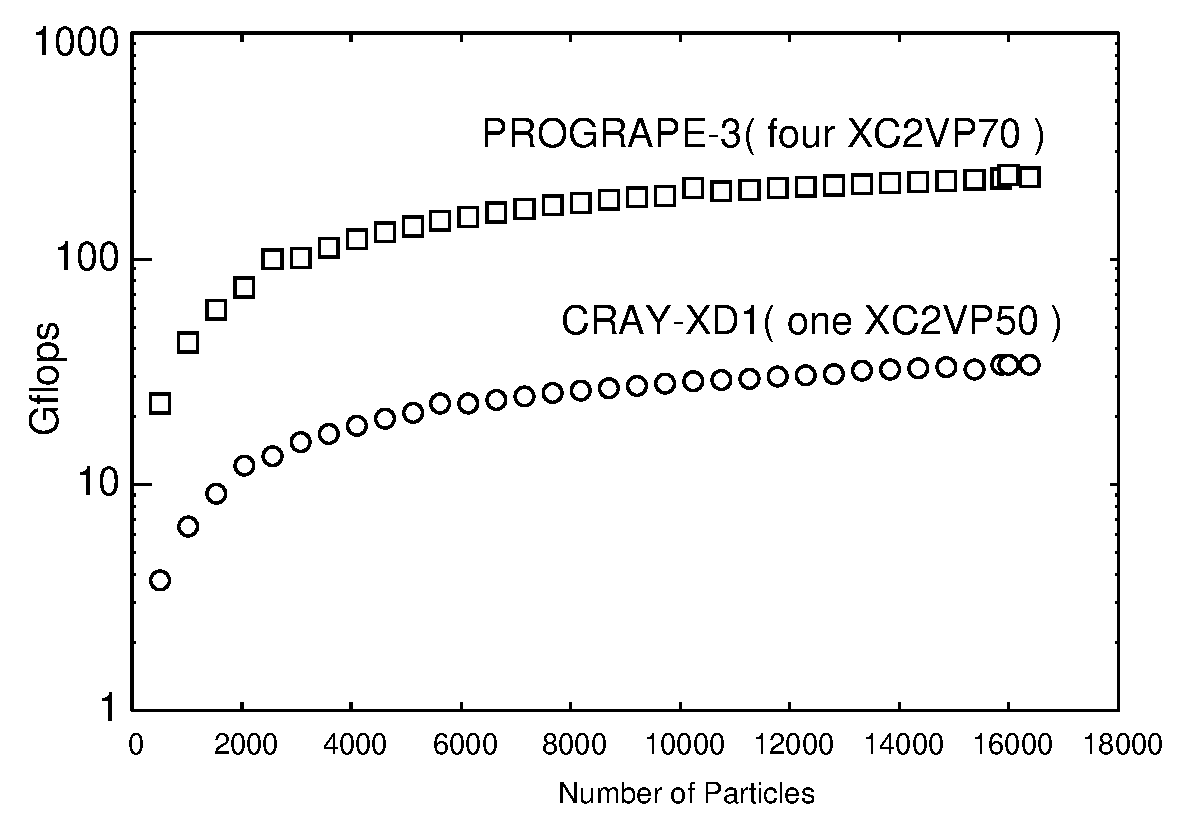
\includegraphics[angle=+0,width=8cm]{./mat/perform/graph.eps}
\caption{The mesured caluclation speed of single PROGRAPE-3 board in Gflops for the direct-summation algorithm, plotted as functions of the number of particles, N.}
\label{MESURE-PERFORM}
\end{center}
\end{figure}


\section{Related work}

There have been several investigations of parametrized floating point
arithmetic IP cores. \cite{JL01,LCCN03} presented prametrized floating
point adders and multipliers. \cite{LKM02,WN04} presented parametrized
floating point square roots and divisions. In most of these works, the
square root and divisions are implemented using subtractors and
shifters. This way is not suitable for pipelined implementations
bacause carry propagations of ripple-carry subtractor are given to becoming long and
a lot of pipeline stages are required in an arithmetic unit such as square
root, division. For pipelined implementations, it is better to use
function evaluators using first or second order polynomial
interpolation.

Even if the elementary functions such as square root, division,
$r^{-1.5}$ or $log_{2}(1+2^{-x})$ etc are implemented using function
evaluators, it can not by said these implementations are enough.  If
someone uses cofficients table from taylor expanded polynomials, the
situation becomes serious. Residual errors of an approximate value in a section

taylor Residual errors in a section .

\begin{figure}[htb]
\begin{center}
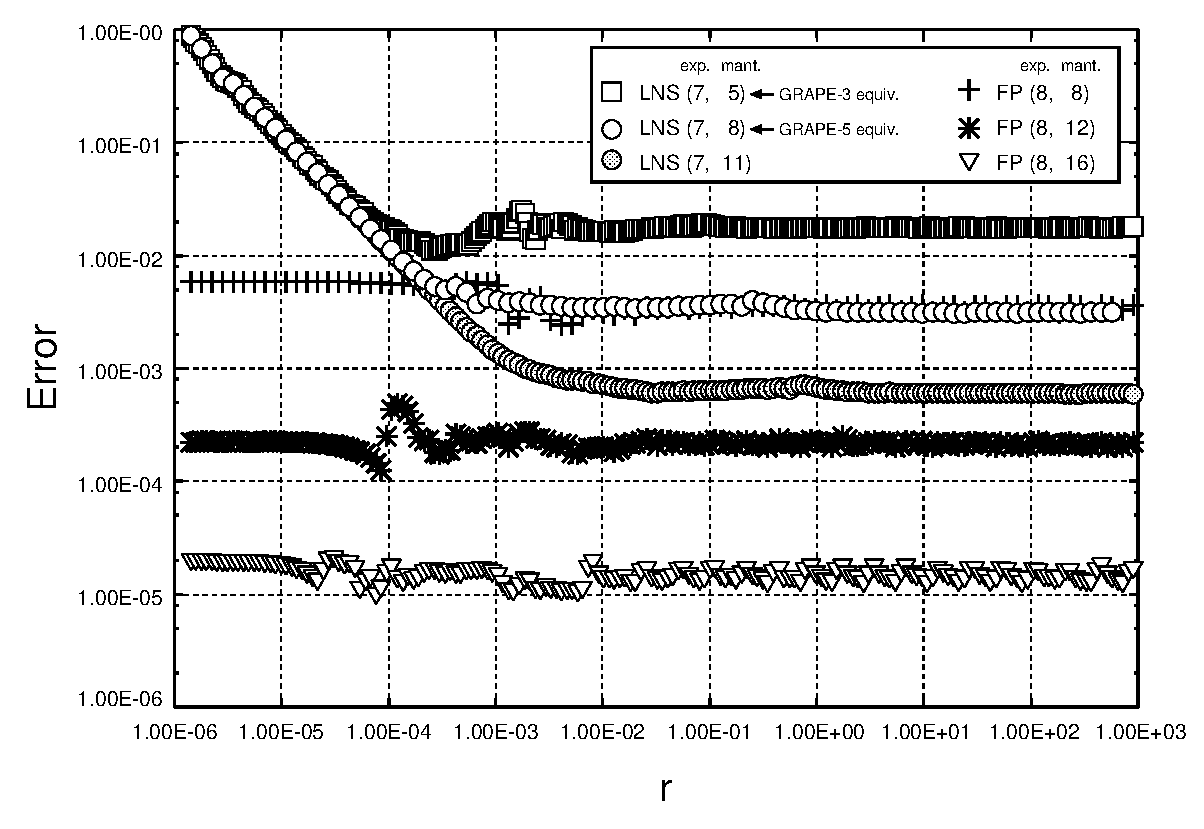
\includegraphics[angle=+0,width=13cm]{./mat/SrGraph.eps}
\caption{Quantization error for froce calculation in the N-body problem.}
\label{SrError}
\end{center}
\end{figure}



Lee\cite{XXX}

%%PROGRAPE-1
An earlier example of the use of reconfigurable hardware in the
acceleration of scientific computations is PROGRAPE-1(PROgrammable
GRAPE-1)\ref{HFKM00}. PROGRAPE-1 is an FBA for many-body
simulations. It is implemented with two Altera EPF10K100 FPGAs, each
of which contains about 100k gates. The peak performance of
calculating gravitational force results in 0.96 Gflops.  PROGRAPE-1
was composed of short length(14-bit) logarithmic arithmetics and this
was the reason why the performance was excelent with this outdated
FPGAs.

%%RACE
MPRACE\footnote{\tt http://www-li5.ti.uni-mannheim.de/fpga/race/} is
similar system to PROGRAPE-1, which uses a parameterized
floating-point library\cite{LKM02}.  The target application of MPRACE
is astrophysical hydrodynamics simulations using SPH(Smoothed Particle
Hydrodynamics) method.  They are making an effort to construct a high
performance system.


%%CAST
CAST(Computer Arithmetic Synthesis Tool)\ref{THYL04} is a similar tool
to our PGR.  The contribution of both tools is a set of parametrized
floating-point, fixed-point, and logarithmic numbers libraries and a
tool that generates a computational pipeline from an abstract description.
The CAST developers claimed that they have implemented
a pipeline for gravitational N-body problem. 
However, they have only indicated 
projected results based on simulation with only one pipeline unit.
There is a big distance between implementing a pipeline unit and building a real
high-performance commutating system. In contrast to their work,
we have implemented 64 pipelines (16 pipelines per one FPGA chip)
for gravitational N-body problem on our target hardware PROGRAPE3 board,
and the mesured highest performance of our system
(Opteron 2.4GHz PC + one PROGRAPE-3 board) is 100 GFLOPS as shown in Figure \ref{MESURE-PERFORM}.
We have proved a real high-performance computing system
can be implemented using the PGR.

%%MARGE

\section{Conclusion}
We have developed the PGR package, a software which automatically generate
most of communication softwares and the hardware descriptions
(the bit-level hardware design of pipeline processors)
for FBAs from a high-level description PGDL.
Using the PGR package, we have implemented gravitational force
pipelines used in astrophysical simulations.
The PGDL description for the gravitational force pipelines
is only a several tens of lines of a text file.
Regardless of a very simple description, we could obtain very
efficient implementation. 
Using PGR, we will reach the design area where nobody can achieve.

%------------------------------------------------------------------------- 
\bibliographystyle{latex8}
\begin{thebibliography}{}

\bibitem{AKEDC04}
Azizi, N., Kuon, I., Egier, A., Darabiha, A., \& Chow, P.:
Reconfigurable Molecular Dynamics Simulator.
Proc. of IEEE FCCM'04 Symposium on Field-Programmable Custom Computing Machines, Los Alamitos, CA.
(2004) 197-206

\bibitem{BH98}
Bellows, P., \& Hutchings., B.:
JHDL - An HDL for Reconfigurable Systems.
Proc. of IEEE FCCM'03 Symposium on Field-Programmable Custom Computing Machines, Los Alamitos, CA.
(1998) 175--184

\bibitem{FO01}
Flynn, J., M., \& Oberman, F., S.,:
Advanced Computer Arithmetic Design.
John Wiley \& Sons, New York.
(2001)

\bibitem{GKMK96}
Gokhale, M., Kaba, J., Marks, A., \& Kim, J.:
Malleable architecture generator for FPGA computing.
Proc. SPIE 2914.
(1996) 208--217,

\bibitem{HFKM00}
Hamada,~T., Fukushige,~T., Kawai,~A., \& Makino,~J.:
PROGRAPE-1: A Programmable, Multi-Purpose Computer for Many-Body Simulations.
Publication of Astronomical Society of Japan.
{\bfseries 52} (2000) 943--954

\bibitem{HTYLL03}
Ho, C., Tsoi, K., Yeung, H., Lam, Y., Lee, K., Leong, P., Ludewig, R., Zipf, P., Ortiz, A., \& Glesner, M.:
Arbitrary function approximation in HDLs with application to the n-body problem.
In 2003 IEEE International Conference on Field-Programmable Technology(FPT).
(2003) 84--91

\bibitem{JL01}
Jaenicke, A., \& Luk, A.:
Parametrized Floating-Point Arithmetic on FPGAs.
Proc. of IEEE ICASSP, 
{\bfseries 2} (2001) 897--900

\bibitem{KFMT00}
Kawai,~A., Fukushige,~T., Makino,~J., \& Taiji,~M.:
GRAPE-5: A Special-Purpose Computer for N-body Simulation.
Publication of Astronomical Society of Japan.
{\bfseries 52} (2000) 659--676

\bibitem{LKM02}
Lienhart, G, L., Kugel, A., \& M{\"a}nner, R.:
Using Floating Point Arithmetic on FPGAs to Accelerate Scientific N-Body Simulations.
Proc. of IEEE FCCM'02 Symposium on Field-Programmable Custom Computing Machines, Los Alamitos, CA.
(2002) 182--191

\bibitem{LCCN03}
Leyva, G., Caffarena, G., Carreras, C., \& Nieto-Taladriz, O.:
A Generator of High-speed Floating-point Modules.
Proc. of IEEE FCCM'04 Symposium on Field-Programmable Custom Computing Machines, Los Alamitos, CA.
(2004) 306--307 

\bibitem{LTM03}
Liang, J., Tessier, R., \& Mencer, O.:
Floating Point Unit Generation and Evaluation for FPGAs.
Proc. of IEEE FCCM'03 Symposium on Field-Programmable Custom Computing Machines, Los Alamitos, CA.
(2003) 185--194

\bibitem{MMF97}
Mencer, O., Morf, M. \& Flynn, J., M.:
PAM-Blox: High Performance FPGA Design for Adaptive Computing.
Proc. of IEEE FCCM'98 Symposium on Field-Programmable Custom Computing Machines, Los Alamitos, CA.
(1997) 167--174

\bibitem{M97}
Muller, M., J.:
Elementary Functions: Algorithms and Implementation.
Brikhauser Verlag AG.
(1997)

%\bibitem{MIE90}
%Makino, J., Ito, T., \& Ebisuzaki, T.:
%Error Analysis of the GRAPE-1 Special-Purpose N-Body Machine.
%Publication of Astronomical Society of Japan.
%{\bfseries 42} (1990) 717--736

\bibitem{MT98}
Makino,~J., \& Taiji,~M.:
Scientific Simulations with Special-Purpose Computers --- The GRAPE Systems.
Chichester: John Wiley and Sons.
(1998)

\bibitem{MPMF01}
Mencer, O., Platzner, M., Morf, M. \& Flynn, J., M.:
Object-Oriented Domain-Specific Compilers for Programming FPGAs.
IEEE Trans. on VLSI, special issue on Reconfigurable Computing.
(2001)


\bibitem{OMEFS93}
Okumura, K., S., Makino, J., Ebisuzaki, T. Fukushige, T., Ito, T. \& Sugimoto, D.:
Highly Parallelized Special-Purpose Computer, GRAPE-3.
Publication of Astronomical Society of Japan.
{\bfseries 45} (1993) 329--338


\bibitem{SS99}
Stine, J., \& Schulte, M.:
The symmetric table addition method for accurate function approximation.
In Journal of VLSI Signal Processing.
(1999) 167--177

\bibitem{SS03}
Smith, W., D., \& Schore, A., R.:
Towards an RCC-based accelerator for computational fluid dynamics applications.
Proc. of the 2003 International Conference on Engineering Reconfigurable Systems and Algorithms.
(2003)

\bibitem{THYL04}
Tsoi, K., Ho, C., Yeung, H., \& Leong, P.:
An Arithmetic Library and its Application to the N-body Problem.
Proc. of IEEE Symposium on Field-Programmable Custom Computing Machines, IEEE Computer Society Press.
(2004) 68--78

\bibitem{WN04}
Wang, X.,\& Nelson, B., E.:
Tradeoffs of Designing Floating-Point Division and Square Root on Virtex FPGAs
Proc. of IEEE FCCM'03 Symposium on Field-Programmable Custom Computing Machines, Los Alamitos, CA.
(2004) 195--203


\end{thebibliography}

\end{document}
